\chapter{Introduction}

  This chapter is an introduction to the research project. Section~\ref{sec:background} is the background and motivation for conducting this research. Section~\ref{sec:researchquestions} includes the research questions to be answered in this report. Section~\ref{sec:deliverables} is a description of what will be the deliverables of this research.
  The methods used in this project is described in Section~\ref{sec:methods}. The last section is an overview of the structure according to the chapters included in this report. 

  \clearpage
  \section{Background and Motivation} \label{sec:background}
  In today's society, people tend to spend much time on their mobile devices. Mobile devices are not just tool for communication, but also an essential tool for everyday tasks like reading mail, pay our bills, and keeping up with our social life. Our whole life is contained in one device. When such a small device is so central to our daily lives, it makes it vulnerable.

  Passwords are human-chosen secrets that are connected to you as a person. When creating a password, people tend to create a password that is an association to something they know or recognize; passwords are more than just words and numbers. Because of the shortcomings with text-based passwords \cite{UnixPasswords}, there is an increased interest in graphical passwords. The interest in graphical passwords started by the assumption that pictures are easier to remember and more secure than words and numbers \cite{DeAngeli}.

  The motivation for this thesis began by observing the shortcomings with the text-based authentication. Password reuse is one of the known password habits among users because the human limitation to remembering text-based password. Some users also make simple or meaningful password that are easier to remember, making their passwords vulnerable to attacks. Graphical passwords look like a promising alternative to text-based passwords, as it supports users to remember and make more complex passwords, offering better usability and higher security. As mobile devices play a significant role in our everyday life, it makes it interesting target device. Security on mobile devices has changed during the past years. The history of locking mechanisms was often a solution solely to prevent accidental use, while current mobile phones require protection in order to secure the potentially vast amount of private data that we keep on our mobile devices. The situation of our rapid use of mobile devices, as well as it well-suited platform for graphical password, makes authentication on mobile devices an interesting field of study.

  Google's Android platform released the functionality for the Android Unlock Pattern in 2008. The Android Unlock Pattern is a graphical authentication scheme that enables the users to connect dots as their password. Since its release, there have been much discussion of its security, but few researchers have conducted scientific research on the Android Unlock Pattern. The problem is not just the theoretical password space, but rather the password space in practice. In 2013, a research group conducted the first large-scale user study on the Android Unlock Patterns \cite{Uellenbeck}. The Android Unlock pattern is a screen lock mechanism for the Android mobile operating system. The outcome of the research was an analysis of 2900 user-selected patterns. They found bias in the pattern making process claiming that the scheme are less secure than its stated theoretical password space.

  The aim of this research is to look further into how different user types select their Android Unlock Patterns. This takes previous research a step further by including the human properties that may impact the user's choice in graphical passwords. I believe that graphical passwords are more than just pictures and graphical objects. This thesis is the first phase of my research and will be continued in my master thesis in the following spring.

  \section{Research Questions} \label{sec:researchquestions}
    
  This section contains three research questions to be answered in this research project. They are created based on the introduction and background in Section~\ref{sec:background}. This thesis is the first phase of my research and will be a supporting work for my master thesis that will be a continuation of this project.

  {\bf $RQ1$: What is the status of current research on graphical passwords?} \\
  To answer this research question, there will be conducted a literature review, and will give an overview of the research that is published in the field of graphical passwords. The goal is to find a gap in the research that can be answered in my master thesis as a continuation of this work.

  {\bf $RQ2$: What human properties may affect our choice of graphical passwords on mobile devices?}\\
  My motivation is to find human properties that may impact user's choice in graphical passwords on mobile devices. To answer this, there need to be conducted a review of human properties that describe different user types.

  {\bf $RQ3$: How are we able to collect user-chosen patterns set by various user types?}
  To be able to analyze user-chosen patterns set by different user types, we need to design a prototype for data collection. Collecting user-chosen passwords is not easy to do because people do not give away their passwords easily. When collecting graphical passwords, there is no data source available. It should also be considered how to reach people quickly in order to get a large sample size that can provide statistical significant results in an analysis.

  \section{Deliverables} \label{sec:deliverables}

  There will be three main deliverables in this thesis.

  {\bf Literature review}: The first part of this research is a literature review on graphical passwords. A literature review is providing the information needed to decide on the main research hypothesis for my master thesis, and the aim is to fill the gap in research on graphical passwords on mobile devices.

  {\bf Research design}: The gap found in the literature review will result in a problem domain to be worked in my master thesis. To be able to continue with this work, the research design for next semester will a deliverable of this work. The research design is mainly a detailed description of the research strategy and data collection method.

  {\bf Prototype for data collection}: Research on passwords is not easy to conduct because of the nature of passwords. Passwords should remain a secret for the user, and as we have learned, we should not share our password due to security concerns. Research on text-based passwords is often based on leaked password on the web. When analyzing graphical passwords on mobile devices, there is no such data source available. The prototype can provide insight into a new way of solving the problem of collecting user chosen passwords from mobile devices. This can provide knowledge for future research on graphical passwords on mobile devices. The deliverable will be a suggested prototype for data collection and the data that is desired to collect besides the passwords.

  \section{Methods} \label{sec:methods}

  This section will give a description of the methods used in this research project. 

    \subsection{Research Process} \label{sec:methodresearchprocess}

    Throughout this thesis, the research process illustrated in Figure~\ref{fig:researchProcess1} will be used as a basis for the elaboration of how to conduct the research in my master thesis. The research process is a framework for researching information systems and computing \cite{empiriske}. The only part of the research process that is carried out in this thesis is the background and motivation, as well as the literature review.

      \begin{figure}[H]
        \centering
        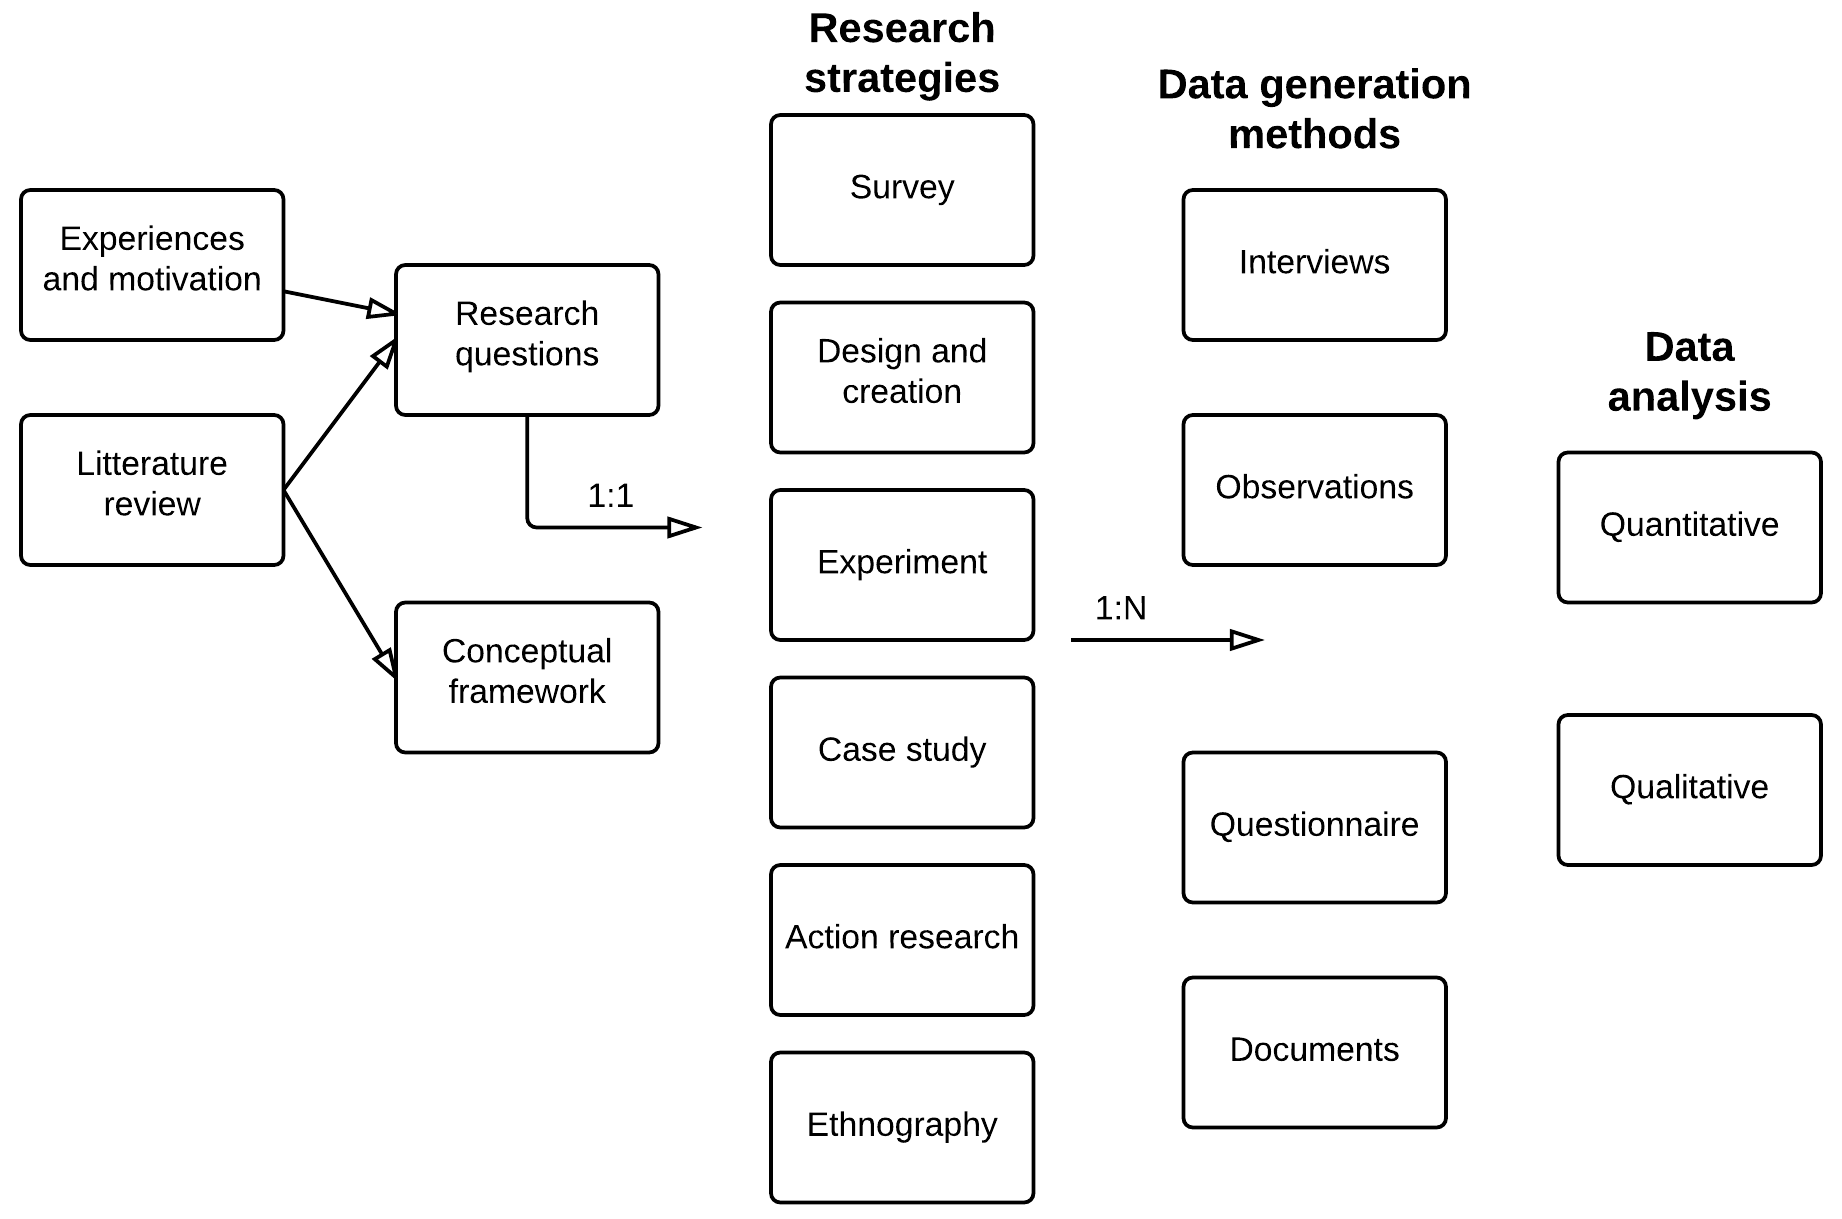
\includegraphics[scale=0.18]{pics/ResearchProcess.png}
        \caption[Research process]{Research Process \cite{empiriske}}
        \label{fig:researchProcess1}
      \end{figure}

    Experiences and motivation is a description of why to conduct the research. A literature review is a review of published research in the selected area of study. By studying the literature, it is given the ability to synthesize it into a coherence account that justifies the chosen research and places it in the context. The literature review should help provide a conceptual framework, that is, the an explicit way of to how I structure the thinking about the research topic and the process undertaking. The conceptual framework includes different factors that comprise the selected topic, the way of thinking about the subject and the way of tackling the research questions. A research strategy is the overall approach to answering the overall hypothesis and research questions. There are six different research strategies: survey, design and creation, experiment, case study, action research, and ethnography. A data generation method how to produce empirical data or evidence. There are four data generation methods: interviews, observation, questionnaire, and documents. Data can either be qualitative or quantitative. 

    \subsection{Literature Review}\label{sec:methodliteraturereview}

    A literature review is often used for two main purposes. {\it First}, by exploring the research, it is useful to look for a suitable research idea and discover relevant material about any possible research topics. {\it Second}, the second part often begin once a research topic is chosen, where the aim is to gather and present evidence to support that the research can produce new knowledge.

    There is a broad range of sources to be used in the literature review, for example, books, journal articles, and conference papers. Books are often based on well know facts with a broad scope. Journal articles and conference papers are more exploratory and are useful for finding information on the current thinking and research in the area. All published journals and conference proceedings needs to be reviewed carefully. It is important to use the sources that is considered to publish quality research and that they provide sufficient quality control on the published research. Some highly rated journals in information systems and computing is: ACM \cite{ACM}, IEEE \cite{IEEE}, and Springer \cite{Springer}. When using conference papers, it can often be useful to read something about their review procedures and their quality requirements. Besides the publication source, it can be helpful to look at the number of citations used. If a research paper has many citations, it may be an indication of it quality.

    When reviewing the literature, it would be too time consuming to read all the papers from the start to the end. To be able to select relevant research, it is preferable to look at the abstract first that should include information about the research motivation, the methods used, as well as the results. If the abstract were promising, I would continue reading the results, and methods used. If the research is very interesting, it might be valuable to read the whole publication.

    Before searching for relevant literature, it is important to define keywords that can narrow the search down to obtain information that is relevant according to the research that is being conducted. The keywords can be combined when searching in different digital libraries.

    When relevant literature is found, it is important to set a list of quality criteria that until now have been discussed.
    The selected quality criteria that are chosen is listed in Table~\ref{tab:QualityCriteria}.

      \begin{table}[H]
        \centering
        \begin{tabular}{| l | p{10cm} |}
          \hline
          {\bf \#} & {\bf Quality Criteria} \\ \hline
          QC 1 & The research is published in a known digital library, journal or conference\\ \hline
          QC 2 & There is a clear statement of the aim of the research\\ \hline
          QC 3 & The study is cited by other researchers\\ \hline
          QC 4 & There is a clear description of the method used in the study\\ \hline
          QC 5 & If the research includes an experiment, user study, or other research strategies, there should be a reasonable sample size used. \\ \hline
        \end{tabular}
        \caption{Quality criteria for literature review}
        \label{tab:QualityCriteria}
      \end{table}
    
    \subsection{Prototyping} \label{sec:methodusabilitytesting}
    The prototype that is being created needs to be evaluated according to usability requirements. For designing the prototype, there is used an design cycle (Figure~\ref{fig:cycle}). {\it First}, there is created a design. {\it Second}, according to the selected design, the design is put into a prototype. When the prototype is not yet implemented, the prototype is illustrated in wireframes. The wireframes are low-level sketches that are inexpensive to create because it requires less time than a technical implementation. {\it Third}, the prototype somehow needs to be evaluated according to usability requirements (further explained in Section~\ref{sec:usability}). The evaluation can be a presentation to people with an interest in this research and from them receiving feedback. An another way to evaluate the prototype is to perform a usability test on a number of users from the population. Results from presentation or test will provide valuable information that is used to redesign the prototype. This is a cycle that will be performed until I reach a design that I am satisfied with. Satisfaction can be measured through usability measures.

    \begin{figure}[H]
      \centering
      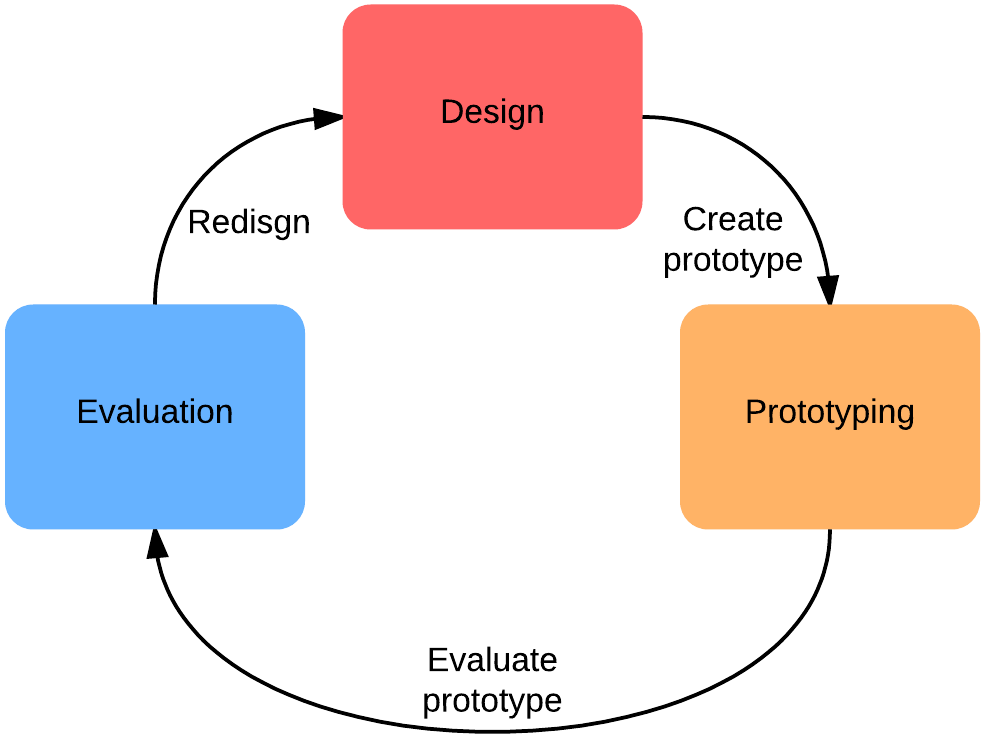
\includegraphics[scale=0.25]{pics/DesignCycle.png}
      \caption[Design Cycle \cite{Norman}]{Design Cycle}
      \label{fig:cycle}
    \end{figure}

  \section{Thesis structure} \label{sec:structure}

    {\bf Chapter 2: An Introduction to Authentication Mechanisms} presents information about authentication, the background and theory for this thesis. 

    {\bf Chapter 3: Literature Review} provides an overview of the current research on graphical passwords. 

    {\bf Chapter 4: Research Design} present the chosen research strategy and data collection method that will be used in my master thesis. 

    {\bf Chapter 5: Further Work} is a summary of further work need to be conducted for a continuation of the work presented in previous chapters.   

